\documentclass[aspectratio=169]{beamer}

% Tema y colores
\usetheme{Madrid}
\usecolortheme{whale}
\definecolor{loyolablue}{RGB}{0,102,153}
\setbeamercolor{structure}{fg=loyolablue}
\setbeamercolor{title}{fg=white,bg=loyolablue}
\setbeamercolor{frametitle}{fg=white,bg=loyolablue}

% Paquetes
\usepackage[utf8]{inputenc}
\usepackage[spanish]{babel}
\usepackage{graphicx}
\usepackage{booktabs}
\usepackage{tikz}
\usepackage{amsmath}

% Quitar navegación
\setbeamertemplate{navigation symbols}{}

% Info
\title[Clasificación de Lesiones Cutáneas]{Clasificación de Lesiones Cutáneas con Deep Learning y Machine Learning}
\subtitle{Ensemble de CNNs para Diagnóstico de Cáncer de Piel}
\author{David Moreda Amezcua \and Javier Cerón Contreras \and Pedro Martínez Huertas}
\institute{Máster Universitario en Inteligencia Artificial\\Universidad Loyola}
\date{Curso 2025/2026}

\begin{document}

% ============================================
% PORTADA
% ============================================
\begin{frame}
    \titlepage
\end{frame}

% ============================================
% DIAPOSITIVA 1: PROBLEMA Y DATOS
% ============================================
\begin{frame}{El Problema: Clasificación de Cáncer de Piel}

    \begin{columns}[T]
        \begin{column}{0.55\textwidth}
            \textbf{Objetivo:} Clasificar imágenes dermoscópicas en 6 tipos de lesiones cutáneas

            \vspace{0.3cm}
            \textbf{Dataset ISIC:}
            \begin{itemize}
                \item Train: 500 imágenes
                \item Validación: 130 imágenes
                \item Test: 161 imágenes
            \end{itemize}

            \vspace{0.3cm}
            \textbf{Desafío principal:}
            \begin{itemize}
                \item Clases muy desbalanceadas
                \item \textcolor{red}{\textbf{MEL (Melanoma):}} solo $\sim$35 imágenes de entrenamiento
                \item Melanoma = clase crítica (mortalidad)
            \end{itemize}
        \end{column}

        \begin{column}{0.42\textwidth}
            \small
            \begin{tabular}{ll}
                \toprule
                \textbf{Clase} & \textbf{Tipo} \\
                \midrule
                ACK & Queratosis Actínica \\
                BCC & Carcinoma Basocelular \\
                \textcolor{red}{MEL} & \textcolor{red}{Melanoma} \\
                NEV & Nevus Melanocítico \\
                SCC & Carcinoma Escamoso \\
                SEK & Queratosis Seborreica \\
                \bottomrule
            \end{tabular}

            \vspace{0.5cm}
            % Placeholder para imagen de ejemplo
            \begin{center}
                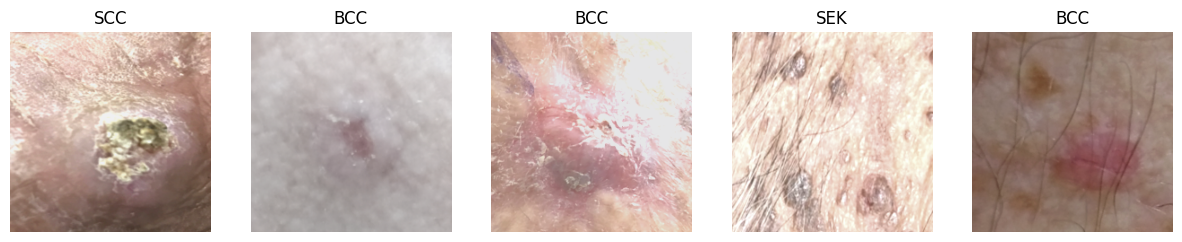
\includegraphics[width=0.9\textwidth]{figuras/ejemplos_dataset_data_augmentation.png}
            \end{center}
        \end{column}
    \end{columns}

\end{frame}

% ============================================
% DIAPOSITIVA 2: METODOLOGÍA
% ============================================
\begin{frame}{Metodología: Ensemble de 3 CNNs}

    \begin{columns}[T]
        \begin{column}{0.6\textwidth}
            \textbf{Arquitecturas utilizadas:}

            \vspace{0.2cm}
            \begin{itemize}
                \item \textbf{ResNet-18:} Conexiones residuales, 11M parámetros
                \item \textbf{DenseNet-121:} Conexiones densas, 7M parámetros
                \item \textbf{YOLO26x-cls:} Estado del arte, backbone potente
            \end{itemize}

            \vspace{0.3cm}
            \textbf{Técnicas aplicadas:}
            \begin{itemize}
                \item Transfer Learning (pesos ImageNet)
                \item Data Augmentation agresivo
                \item Pérdida ponderada por clase
                \item Dropout (0.5) + Weight Decay (0.01)
                \item Early Stopping (paciencia: 15)
            \end{itemize}
        \end{column}

        \begin{column}{0.38\textwidth}
            \textbf{Ensemble (Soft Voting):}

            \vspace{0.3cm}
            \begin{center}
            \begin{tikzpicture}[scale=0.7, transform shape]
                \node[draw, fill=blue!20, rounded corners, minimum width=2cm] (r) at (0,2) {ResNet-18};
                \node[draw, fill=green!20, rounded corners, minimum width=2cm] (d) at (0,1) {DenseNet-121};
                \node[draw, fill=orange!20, rounded corners, minimum width=2cm] (y) at (0,0) {YOLO26x};

                \node[draw, fill=loyolablue!30, rounded corners, minimum width=2.5cm] (e) at (3.5,1) {Ensemble};

                \draw[->, thick] (r) -- node[above, font=\tiny] {20\%} (e);
                \draw[->, thick] (d) -- node[above, font=\tiny] {20\%} (e);
                \draw[->, thick] (y) -- node[below, font=\tiny] {60\%} (e);
            \end{tikzpicture}
            \end{center}

            \vspace{0.3cm}
            \small
            $$\hat{y} = \arg\max \sum_{i} w_i \cdot p_i(c)$$

            \vspace{0.2cm}
            \textit{YOLO domina por mejor rendimiento individual}
        \end{column}
    \end{columns}

\end{frame}

% ============================================
% DIAPOSITIVA 2.5: EXPERIMENTOS ADICIONALES
% ============================================
\begin{frame}{Comparativa de Modelos por Profundidad}

    \begin{columns}[T]
        \begin{column}{0.55\textwidth}
            \textbf{Evaluación de Modelos más Profundos:}
            \vspace{0.2cm}
            \begin{itemize}
                \item Se compararon \textbf{ResNet-50} y \textbf{DenseNet-161} frente a sus versiones ligeras.
                \item \textbf{Resultados:} Disminución del rendimiento en las arquitecturas más profundas.
                \item \textbf{Justificación Técnica:} El dataset limitado (500 imágenes) provoca \textbf{overfitting} prematuro en modelos con alta capacidad, impidiendo una correcta generalización.
            \end{itemize}

            \vspace{0.3cm}
            \begin{block}{Selección Final}
                \small
                Se seleccionan ResNet-18 y DenseNet-121 por ofrecer el mejor balance entre capacidad de aprendizaje y generalización.
            \end{block}
        \end{column}

        \begin{column}{0.42\textwidth}
            \textbf{Comparativa de Rendimiento (Test):}
            \vspace{0.2cm}
            \begin{table}
                \small
                \centering
                \begin{tabular}{lcc}
                    \toprule
                    \textbf{Modelo} & \textbf{Acc} & \textbf{F1} \\
                    \midrule
                    \rowcolor{green!20} \textbf{ResNet-18} & \textbf{58.4\%} & \textbf{0.58} \\
                    ResNet-50 & 52.2\% & 0.52 \\
                    \midrule
                    \rowcolor{green!20} \textbf{DenseNet-121} & \textbf{59.0\%} & \textbf{0.59} \\
                    DenseNet-161 & 54.0\% & 0.53 \\
                    \bottomrule
                \end{tabular}
            \end{table}
            \vspace{0.1cm}
            \centering\footnotesize\textit{Menos parámetros = Mejor generalización}
        \end{column}
    \end{columns}

\end{frame}

% ============================================
% DIAPOSITIVA 3: RESULTADOS
% ============================================
\begin{frame}{Resultados del Ensemble}

    \begin{columns}[T]
        \begin{column}{0.48\textwidth}
            \textbf{Métricas Globales:}

            \vspace{0.3cm}
            \begin{tabular}{lc}
                \toprule
                \textbf{Métrica} & \textbf{Valor} \\
                \midrule
                Accuracy & 62.7\% \\
                \textbf{F1-Macro} & \textbf{0.63} \\
                Cohen's Kappa & 0.55 \\
                \bottomrule
            \end{tabular}

            \vspace{0.5cm}
            \textbf{Resultado Crítico - Melanoma:}

            \vspace{0.2cm}
            \begin{tabular}{lc}
                \toprule
                \textbf{Métrica MEL} & \textbf{Valor} \\
                \midrule
                \textcolor{red}{Precisión} & \textcolor{red}{\textbf{100\%}} \\
                Recall & 71\% \\
                F1-Score & 0.71 \\
                \bottomrule
            \end{tabular}

            \vspace{0.2cm}
            \small\textit{Sin falsos positivos de melanoma}
        \end{column}

        \begin{column}{0.48\textwidth}
            \textbf{F1-Score por Clase:}

            \vspace{0.3cm}
            \begin{tabular}{lcc}
                \toprule
                \textbf{Clase} & \textbf{F1} & \textbf{Soporte} \\
                \midrule
                ACK & 0.50 & 22 \\
                BCC & 0.68 & 30 \\
                \textcolor{red}{MEL} & \textcolor{red}{0.71} & 17 \\
                NEV & 0.75 & 27 \\
                SCC & 0.47 & 21 \\
                SEK & 0.65 & 44 \\
                \midrule
                \textbf{Macro} & \textbf{0.63} & 161 \\
                \bottomrule
            \end{tabular}

            \vspace{0.3cm}
            % Placeholder para matriz de confusión
            \begin{center}
                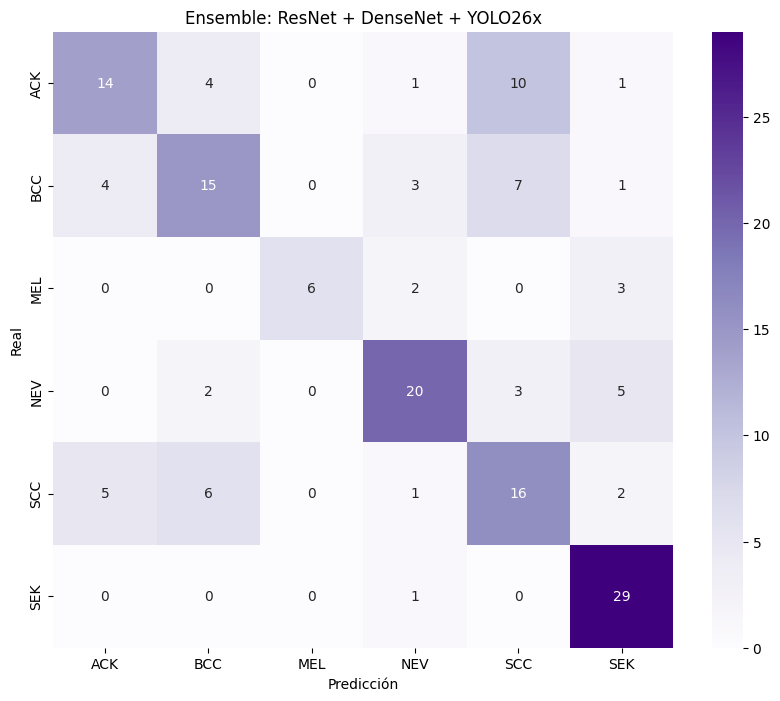
\includegraphics[width=0.8\textwidth]{figuras/ensemble_confmat.png}
            \end{center}
        \end{column}
    \end{columns}

\end{frame}

% ============================================
% DIAPOSITIVA 4: CONCLUSIONES
% ============================================
\begin{frame}{Conclusiones}

    \begin{columns}[T]
        \begin{column}{0.55\textwidth}
            \textbf{Logros:}
            \begin{itemize}
                \item Ensemble supera a modelos individuales
                \item \textcolor{red}{\textbf{100\% precisión en Melanoma}} (clase crítica)
                \item F1-Macro de 0.63 con solo 500 imágenes
                \item YOLO26x mejor modelo individual
            \end{itemize}

            \vspace{0.4cm}
            \textbf{Limitaciones:}
            \begin{itemize}
                \item Dataset pequeño (500 train)
                \item Clases minoritarias difíciles (ACK, SCC)
                \item Ceiling impuesto por cantidad de datos
            \end{itemize}
        \end{column}

        \begin{column}{0.42\textwidth}
            \textbf{Contribución de cada modelo:}

            \vspace{0.3cm}
            \begin{center}
            \begin{tikzpicture}[scale=0.8]
                % Barras horizontales simples
                \fill[blue!60] (0,2) rectangle (2.4,2.4);
                \node[right] at (2.5,2.2) {\small ResNet: 58\%};

                \fill[green!60] (0,1.2) rectangle (2.5,1.6);
                \node[right] at (2.6,1.4) {\small DenseNet: 59\%};

                \fill[orange!60] (0,0.4) rectangle (3.0,0.8);
                \node[right] at (3.1,0.6) {\small YOLO: 60\%};

                \fill[loyolablue!80] (0,-0.4) rectangle (3.1,-0.0);
                \node[right] at (3.2,-0.2) {\small \textbf{Ensemble: 63\%}};
            \end{tikzpicture}
            \end{center}

            \vspace{0.5cm}
            \begin{block}{Trabajo Futuro}
                \small
                Ampliar dataset, probar Vision Transformers, optimizar pesos del ensemble
            \end{block}
        \end{column}
    \end{columns}

\end{frame}

\end{document}
